\documentclass[11pt, letterpaper]{article}   	% use "amsart" instead of "article" for AMSLaTeX format
\usepackage{graphicx}				% Use pdf, png, jpg, or eps§ with pdflatex; use eps in DVI mode
\usepackage{amssymb}
\usepackage{amsmath}
\usepackage{url}
% Allow inline lists
\usepackage[inline]{enumitem}
\usepackage[backend=biber, style=authoryear, autocite=inline, isbn=false, doi=false, url=false, eprint=false]{biblatex}
% Fix biblatex behavior that writes "In: " before journal name.
\renewbibmacro{in:}{%
  \ifentrytype{article}{}{\printtext{\bibstring{in}\intitlepunct}}}


\newcommand{\eq}[1]{Eq.~(\ref{#1})}
\newcommand{\Eq}[1]{Equation~(\ref{#1})}
\newcommand{\eqs}[2]{Eq.~(\ref{#1})~and~(\ref{#2})}
\newcommand{\fig}[1]{Fig.~\ref{#1}}
\newcommand{\Fig}[1]{Figure~\ref{#1}}
\newcommand{\figs}[2]{Fig.~\ref{#1}~and~\ref{#2}}

\newcommand{\floor}[1]{\lfloor #1 \rfloor}
\newcommand{\E}[1]{\left< #1 \right>}

\DeclareMathOperator{\pmi}{pmi}
\DeclareMathOperator{\fpmi}{fpmi}
\DeclareMathOperator{\wfpmi}{wfpmi}
\DeclareMathOperator{\hilopmi}{hilopmi}


\bibliography{references}

\title{Distinguishing among coalescent models using two-site allele frequency spectra}
\author{Daniel P. Rice}
\date{\today}

\begin{document}
\maketitle

\abstract{[NOTE: OLD]
The genetic diversity of a population reflects its demographic and
evolutionary history. Methods for inferring this history typically
assume that the ancestry of a sample can be modeled by the Kingman
coalescent process. A defining feature of the Kingman coalescent is
that it generates genealogies that are binary trees: no more than two
ancestral lineages may coalesce at the same time. However, this
assumption breaks down under several scenarios. For example, pervasive
natural selection, rapid spatial range expansion, and extreme
variation in offspring number can all generate genealogies with
``multiple-merger'' events in which more than two lineages coalesce
instantaneously. Therefore, detecting multiple mergers is important
both for understanding which forces have shaped the diversity of a
population and for avoiding fitting misspecified models to data.
Current methods to detect multiple mergers rely on the average site
frequency spectrum (SFS). However, the signatures of multiple
mergers in the average SFS are also consistent with a Kingman
coalescent process with a time-varying population size. Here, I
present a new method for detecting multiple mergers based on
the mutual information of the joint allele frequency spectrum at pairs of linked sites. Unlike the average SFS,
the mutual information depends mostly on the topologies of genealogies
rather than their branch lengths and is therefore robust to most
demographic effects.}

\section*{Introduction}
The genetic diversity of a population reflects its demographic and evolutionary history.
Learning about this history from contemporary genetic data is the domain of modern population genetics (see~\cite{Hahn2018a}).
The fundamental tools of the trade are simplified mathematical models, which connect unobserved quantities such as the population size to observable features of genetic data.
However, populations are complicated and, moreover, varied in their complications.
No simple model can capture the processes governing every species' evolution, and fitting a misspecified model will generate misleading inferences.
It is therefore crucial to understand the limits of our models and to be able to assess when a model is appropriate for a particular data set.

One of the most widely used models is the Kingman coalescent~\autocite{Kingman1982a, Kingman1982b, Kingman1982c, Hudson1983, Tajima1983}.
The Kingman coalescent is a stochastic process that generates gene genealogies, trees representing the patterns of shared ancestry of sampled individuals.
Inference methods use these genealogies as latent variables linking demographic parameters to genetic data~\autocite{RosenbergNordborg2002}.
The Kingman coalescent has a number of convenient properties that allow for both analytical calculations (e.g.,~\cite{Tajima1989}) and efficient stochastic simulations (e.g.,~\cite{Hudson2002}): tree topologies are independent of waiting times; waiting times are generated by a Markov process; and neutral mutations are modeled as a Poisson process conditionally independent of the tree.
Moreover, the model may be extended to study a variety of biological phenomena including recombination, population structure, and variation in sex ratios or ploidy (see generally~\cite{Wakeley2009}).

An important application of the Kingman coalescent is inferring historical population sizes from genetic data~\autocite{SchraiberAkey2015}.
In its simplest form, the model has a single parameter, the coalescent rate, which determines the branch lengths of genealogies~\autocite{Kingman1982a}.
Under a variety of conditions, the coalescent rate is inversely proportional to the population size~\autocite{Kingman1982b}.
Accordingly, a growing or shrinking population may be modeled by a time-varying rate~\autocite{GriffithsTavare1994, GriffithsTavare1998}.
Patterns of genetic diversity depend on the ratio of the coalescent rate to other evolutionary rate parameters.
For example, the \emph{site frequency spectrum} (SFS)---the number of mutations segregating at different frequencies in a sample---is determined by the ratio of the mutation rate to the (time-varying) coalescent rate.
Kingman coalescent--based inference methods solve the inverse problem of determining the population size history that best explains particular features of the data, such as the SFS (e.g., \cite{BhaskarEtAl2015}) or variations in heterozygocity along a chromosome (e.g., \cite{LiDurbin2011}).

A serious problem for this class of inference methods is that different models of evolution generate different relationships between historical population sizes and genetic diversity.
One of the basic assumptions of the Kingman coalescent is that natural selection is negligible in determining the distribution of genealogies.
When this assumption is violated, Kingman-based inference methods are misspecified.
For example, when a beneficial mutation increases rapidly in frequency, it distorts the genealogies at nearby sites (see e.g., \cite{CoopRalph2012}).
If these ``selective sweeps'' occur regularly, they may be the dominant factor determining the distribution of genealogies.
In this case, the average coalescent rate is proportional to the number of beneficial mutations introduced per generation, which is itself \emph{directly} rather than inversely proportional to the population size.
It follows that the relationship between the population size and the expected number of neutral mutations in a sample is inverted: larger populations will be less diverse than smaller populations.

While the example above is extreme, it is well-established that violations of the neutrality assumption can distort or mask the signatures of population size changes.
For example, \cite{SchriderEtAl2016} recently demonstrated that several popular inference methods give misleading results in the presence of selective sweeps.
In a similar vein, \cite{CvijovicEtAl2018}, showed that purifying selection at linked sites that is sufficient to reduce genetic diversity is also sufficient to distort the SFS, leading to a false signal of population growth.
Moreover, genomic evidence from multiple species suggests that such violations of neutrality may be widespread \autocite{SellaEtAl2009, Corbett-DetigEtAl2015, KernHahn2018}.

An important extension of the Kingman coalescent is a family of models known as \textit{multiple merger coalescents} \autocite{Pitman1999, Sagitov1999, DonnellyKurtz1999,} (reviewed in \cite{Eldon2016}), which arise in a variety of contexts both with and without selection.
Whereas in the Kingman coalescent lineages may coalesce only pairwise, multiple merger coalescents permit more than two lineages to coalesce in a single event.
The even more general class of simultaneous multiple merger coalescents \autocite{Schweinsberg2000, MohleSagitov2001, Sagitov2003} permits more than one distinct multiple merger event at the same time.
These models are relevant for species with
``sweepstakes'' reproductive events \autocite{EldonWakeley2006, SargsyanWakeley2008},
fat-tailed offspring number distributions \autocite{Schweinsberg2003},
recurring selective sweeps at linked sites \autocite{DurrettSchweinsberg2005, CoopRalph2012},
rapid adaptation \autocite{NeherHallatscheck2013, DesaiEtAl},
and purifying selection at sufficiently dense sites \autocite{Seger, Good, Nicholaisen}.

In each of these contexts, the coalescent timescale is not necessarily proportional to the population size.
For example, with fat-tailed offspring distributions the rate of coalescence is a power law in the population size \autocite{Schweinsberg2003}, while with linked sweeps it is determined by rate of linked sweeps, as described above \autocite{DurrettSchweinsberg2005}.
In these settings, interpreting the level of genetic diversity in terms of an ``effective population size'' is misleading and inferences based on the Kingman coalescent may be qualitatively incorrect.

It is therefore important to determine whether the Kingman model is appropriate for a given data set before performing demographic inference.
This task is distinct from ``selection scan'' methods designed to detect particular regions of the genome that are under selection (see~\cite{VittiEtAl2013}).
These methods typically assume that most of the genome is evolving neutrally and that the genome-wide distribution of summary statistics reflects demographic factors.
Genomic regions that are outliers from this distribution are presumed to be under selection.
In contrast, we are interested in detecting when the genome-wide background \emph{is not} well-modeled by the Kingman coalescent.

One approach to identifying multiple mergers in genomic data is to use the SFS as a summary statistic.
\cite{BirknerEtAl2013, BlathEtAl2016, SpenceEtAl2016} derived methods for computing the expected site frequency spectrum of (simultaneous-)multiple merger coalescents.
\cite{EldonEtAl2015} showed that it is possible to distinguish between a multiple merger coalescent of the beta family and the Kingman coalescent with exponential growth using the SFS.
\cite{RodelspergerEtAl2014} detected non-Kingman signatures of widespread linked selection in the nematode \textit{Pristionchus pacificus} by demonstrating that the site frequency spectrum is non-monotonic, a signature of multiple mergers \autocite{NeherHallatscheck2013, BirknerEtAl2013}.

However, existing methods have limitations for distinguishing multiple mergers from general models of population-size change.
The primary signature of multiple mergers in the SFS is an overabundance of low-frequency mutations relative to the Kingman expectation, which is also the signature of population growth.
\cite{EldonEtAl2015} were able to reject exponential growth in favor of multiple mergers with sufficient data, but a more flexible model of growth may be able to fit the multiple mergers SFS (see \cite{MyersEtAl2008, BhaskarSong2014}).
The non-mononotic SFS identified by \cite{RodelspergerEtAl2014} is a more robust signature of multiple mergers, but detecting it in data requires knowledge of the ancestral allele at each site.
High-frequency mutations are typically much rarer than low-frequency mutations, so misidentifying even a small fraction of ancestral alleles can generate a non-monotonic SFS at high frequencies.

Here, we propose that summary statistics based on the two-site frequency spectrum (2-SFS)---the generalization of the SFS to pairs of nearby sites \autocite{Hudson2001, FerrettiEtal2018})---are useful for distinguishing between the Kingman coalescent with population growth and multiple merger coalescents.
In particular, we demonstrate that a transformation of the 2-SFS that we refer to as \emph{frequency pointwise mutual information} (fpmi) is sensitive to multiple mergers but relatively invariant under time-varying coalescent rates.
We show that this is true for both perfectly linked sites and sites separated by a moderate genetic distance.
These statistics may be calculated efficiently from genomic single nucleotide polymorphism data.
Furthermore, they do not require phasing, recombination maps, or ancestral allele identification and are informative even with small sample sizes.
Together, these properties make the 2-SFS useful for demographic model-checking in a wide range of species.
We demonstrate this model-checking procedure on genomic diversity data from \textit{Drosophila melanogaster} \autocite{LackEtAl2015}.

Following the notation of \cite{Fu1995}, the site frequency spectrum of a sample of $n$ haploid genomes is $\left\{ \xi_i : 1 \leq i < n \right\}$, where $\xi_i$ is the fraction of sites containing a mutation with derived allele count $i$ in the sample.
In many cases, the ancestral allele is unknown and so the allele in $i$ samples and the complimentary allele in $n-i$ samples are indistinguishable.
Therefore, we will mostly consider the \textit{folded} site frequency spectrum $\left\{ \eta_i = \xi_i + (1-\delta_{i,n-i}) \xi_{n-i}: 1 \leq i \leq \floor{n/2} \right\}$, where $\delta_{k,k'}$ is the Kronecker delta. %, where $\eta_i = \xi_i + \delta_{n-2i} \xi_{n-i}$.
The SFS and folded SFS can be calculated from a set of single nucleotide polymorphisms (SNPs) without any information about their relative locations in the genome.

In contrast, the 2-SFS is a statistic of \textit{pairs} of sites.
We define the 2-SFS,
$\left\{ \xi_{ij}(d) : d > 0; 1 \leq i, j < n\right\}$,
as the fraction of pairs of sites separated by $d$ bases for which there is a mutation with derived allele count $i$ at one site and a second mutation with derived allele count $j$ at the other site.
(Note that $\xi_{ij}(d) = \xi_{ji}(d)$ by symmetry.)
This object has been studied for non-recombining sites by \cite{FerrettiEtAl2018} in a neutral model and \cite{Xie2011} in a model with selection.
We define the folded 2-SFS, $\eta_{ij}(d)$, by analogy to the folded SFS,  categorizing pairs of sites by their minor allele frequencies.

In the limit of low per-site mutation rate ($\mu\to0$), and no recombination, all polymorphic sites are bi-allelic and the expected SFS and 2-SFS are related to moments of the branch length distribution by
\begin{align}
    \E{\xi_i} &= \mu \E{\tau_i} \label{eq:expected_sfs} \\
    \E{\xi_{ij}} &= \mu^2 \E{\tau_i \tau_j},
    \label{eq:expected_2sfs}
\end{align}
where $\tau_i$ is the total length of branches subtending $i$ leaves of a gene genealogy and $\E{\cdot}$ represents the expectation over the distribution of gene genealogies defined by a coalescent model.
(We suppress the distance, $d$, for non-recombining sites.)
Thus, the SFS and 2-SFS depend on the distribution of coalescent times as well as the distribution of tree topologies.

\cite{Fu1995} calculated the first and second moments of the branch-length distribution for non-recombining infinite sites locus under the standard time-homogeneous Kingman coalescent.
He found that $\E{\tau_i \tau_j} < \E{\tau_i}\E{\tau_j}$ for all $j \not\in \{i, (n-i)\}$.
This result, combined with \eqs{eq:expected_sfs}{eq:expected_2sfs}, implies a negative correlation between mutations at different frequencies: trees generating a mutation with derived allele count $i$ are less likely than average to generate a second mutation with derived allele count $j \not\in \{i, (n-i)\}$.
(There are positive correlations between mutations at complementary frequencies induced by genealogies whose root node partitions the tree into subtrees of size $i$ and $n-i$.)

\cite{BirknerEtAl2013} extended Fu's calculation to a family of multiple merger coalescents called beta coalescents.
This one-parameter family interpolates between the Kingman coalescent and the Bolthausen-Sznitman coalescent as the parameter, $\alpha$, varies from 2 to 1.
Beta coalescents arise in models with fat-tailed offspring distributions \autocite{Schweinsberg2003}, and the Bolthausen-Sznitman coalescent is the limiting distribution of genealogies in rapidly adapting populations \autocite{NeherHallatscheck2013}.
Like Fu, Birkner et al.\ were primarily concerned with computing the sample variance of SFS-based summary statistics such as Tajima's D \autocite{Tajima1989}.
As a result, they were mostly interested in the diagonal terms of the SFS covariance matrix, which dominate that calculation.
However, Figures 5 and 6 of \cite{BirknerEtAl2013} show positive correlations between $\xi_i$ and $\xi_j$ for $j \neq i, n-i$.
Thus, unlike the standard Kingman coalescent, the beta coalescent can generate positive associations between mutations with different minor allele counts.

In the following, we demonstrate that this distinction in the 2-SFS between the multiple merger and Kingman coalescents
\begin{enumerate*}[label=(\roman*), before=\unskip{: }, itemjoin={{; }}, itemjoin*={{, and }}]
    \item applies to Kingman coalescents with time-varying coalescent rates
    \item is robust to recombination between the sites
    \item is also a feature of forward-time models with selection
    \item can form the basis of a model-checking procedure for demographic inference methods
\end{enumerate*}.


\section*{Methods}

\subsection*{Frequency pointwise mutual information}

We are interested in quantifying the dependence between minor allele counts at a pair of sites, particularly for $i\neq j$.
To do so, we define the \textit{frequency pointwise mutual information} as
\begin{align}
    \fpmi(i,j;d) = \log \frac{\E{\eta_{i,j}(d)}}{\E{\eta_i} \E{\eta_j}}.
    \label{eq:fpmi}
\end{align}
\Fig{fig:schematic} shows the steps to compute $\fpmi$ from a sample of sequences.

\begin{figure}
\centering
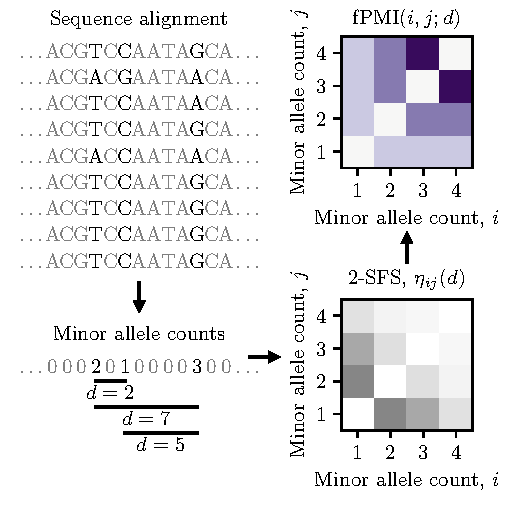
\includegraphics[width=0.5\textwidth]{figures/schematic.pdf}
\caption{Summarizing population genetic data with frequency pointwise information. First, a sequence alignment is reduced to the minor allele frequencies and positions of segregating mutations. Then, for a given distance, $d$, the 2-SFS gives the number of pairs of sites with each combination of minor allele frequencies. Finally, $\fpmi$ is calculated from the 2-SFS according to \eq{eq:fpmi}.
[OPTIONS: Could add (1) weighted fpmi, and/or (2) binned 2-SFS] \label{fig:schematic}}
\end{figure}

In information theory, the pointwise mutual information of a pair of random variables (PMI), $X$ and $Y$, is a transformation of the probability mass function, $p(x,y)$, given by
\begin{align}
    \pmi(x,y) = \log \frac{p(x,y)}{p(x)p(y)} = \log \frac{p(x|y)}{p(x)}
    \label{eq:pmi}
\end{align}
where $p(x) = \sum_y p(x,y)$ and vice versa \autocite{ChurchHanks1990}.
PMI measures the change in the probability that $X=x$ given knowledge that $Y=y$.
When $X$ and $Y$ are independent, $\pmi(x,y) = 0$ for all $x,y$.
On the other hand, when $X$ and $Y$ are not independent, $\pmi(x,y) > 0$ implies that $p(x|y) > p(x)$, and conversely for $\pmi(x,y) < 0$.
(The expectation of PMI over the joint distribution of $X$ and $Y$ is known as the mutual information of $X$ and $Y$ \autocite{CoverThomas1991}.)

In our setting, the 2-SFS may be interpreted as a joint probability mass function over allele frequencies.
Given a coalescent model, the minor allele count at an arbitrary site is a random variable with probability mass function $p(i) = \E{\eta_i}$, where we define $\eta_0$ to be the fraction of monomorphic sites.
Similarly, the minor allele counts at a pair of sites separated by $d$ bases is a pair of random variables with joint probability mass function $p_d(i,j) = \E{\eta_{ij}(d)}$.
Comparing, \eq{eq:fpmi} with \eq{eq:pmi} shows that $\fpmi$ is the standard pointwise mutual information for pairs of allele frequencies.

This transformation of the 2-SFS has several useful properties.
First, because it is based on the minor allele frequencies, we may compute $\fpmi$ from data without knowing the ancestral allele.
Moreover, the results of \cite{Fu1995} show that $\fpmi(i,j) < 0$ for $i\neq j$ for non-recombining sites under the time-homogeneous Kingman coalescent.

The second benefit of computing $\fpmi$ from the 2-SFS is that it normalizes for distortions in the SFS.
Population-size variation distorts the SFS by changing the distribution of waiting times.
However, the time-inhomogeneous Kingman coalescent generates the same distribution of tree topologies as the time-homogeneous version.
On the other hand, multiple mergers alter both the coalescent time distribution and the distribution of topologies.
These two effects are convolved in the SFS, making it difficult to distinguish between population growth and multiple mergers.
Our hope is that the $\fpmi$ reflects additional information about the distribution of genealogies, once distortions in coalescent times are accounted for.
That is, we expect $\fpmi$ to be sensitive to multiple mergers, but invariant under changes in the coalescent rate.

% A general measure of the dependence between a pair of random variables is the \textit{mutual information} \autocite{CoverThomas1991}.
% The mutual information between random variables $X$ and $Y$ is a functional of their joint probability mass function, $p(x,y)$, defined as
% \begin{align}
%     I[p(x,y)] = \sum_{x,y} p(x,y) \log \frac{p(x,y)}{p(x)p(y)},
%     \label{eq:mutual_information}
% \end{align}
% where $p(x) = \sum_y p(x,y)$ and vice versa.
% Equivalently, the mutual information is the Kullback-Leibler divergence between the true joint distribution of $X$ and $Y$ and the joint distribution of two independent random variables with the same marginal distributions as $X$ and $Y$ \autocite{CoverThomas1991}.
% Thus, mutual information captures generic, possibly nonlinear, dependence between $X$ and $Y$.

% We would like to measure the association between alleles at particular frequencies, rather than the overall dependence between allele frequencies at nearby sites (which would be a measure of linkage disequilibrium).
% \Eq{eq:mutual_information} shows that $I[p(x,y)]$ is the expectation, relative to $p(x,y)$, of a quantity known as the \textit{pointwise mutual information}, where
% \begin{align}
%     \pmi(x,y) = \log \frac{p(x,y)}{p(x)p(y)} = \log \frac{p(x|y)}{p(x)} = \log \frac{p(y|x)}{p(y)}
% \end{align}
% \autocite{ChurchHanks1990}.
% Pointwise mutual information measures the change in the probability that $X=x$ given knowledge that $Y=y$.
% When $X$ and $Y$ are independent, $\pmi(x,y) = 0$ for all $x,y$.
% On the other hand, when $X$ and $Y$ are not independent, $\pmi(x,y) > 0$ implies that $p(x|y) > p(x)$, and conversely for $\pmi(x,y) < 0$.


\subsection*{Binned allele frequencies}

With finite data, estimates of the 2-SFS will be noisy.
This is particularly true for $i,j\gg1$ because $\E{\eta_{ij}}$ decays like $(ij)^{-1}$ for the standard Kingman \autocite{Fu1995} and faster with growth or multiple mergers.
We show in Results that a positive association between mutations with high minor allele counts and mutations with low minor allele counts is a signature of multiple mergers.
This suggests a binned SFS and 2-SFS:
\begin{align}
    \eta_{\text{lo}}(i_c) &= \sum_{i=1}^{i_c-1} \eta_i \\
    \eta_{\text{hi}}(i_c) &= \sum_{i=i_c}^{\floor{n/2}} \eta_i \\
    \eta_{\text{hi,lo}}(d; i_c) &= \sum_{i=1}^{i_c-1} \sum_{j=i_c}^{\floor{n/2}} \eta_{ij}(d),
\end{align}
where $i_c$ is an arbitrary cutoff between high and low minor allele frequency.
Binning allows us to estimate the 2-SFS stably for large sample sizes, because we may adjust $i_c$ to ensure a large number of sites in both the high--minor allele count and low--minor allele count bins.

We can also compute the pointwise mutual information in this coarse-grained distribution as
\begin{align}
    \hilopmi(d; i_c) = \log \frac
                                {\E{\eta_{\text{hi,lo}}(d; i_c)}}
                                {\E{\eta_{\text{lo}}(i_c)}  \E{\eta_{\text{hi}}(i_c)}}.
\end{align}
One could similarly calculate five other pointwise mutual information statistics from the binning 2-SFS (e.g., the PMI between monomorphic sites and sites with high minor allele counts), but we will not use these statistics here.
Also, it is possible to define less drastic coarse-graining schemes that strike a balance between sampling noise and preserving more detailed information about allele frequencies.

\subsection*{Weighted $\fpmi$}
For plotting purposes, we will also use a weighted version of the $\fpmi$:
\begin{align}
    \wfpmi(i,j:d) = \frac{\E{\eta_{ij}}}{\mu^2 \E{T_2}^2} \fpmi(i,j;d),
    \label{eq:wfpmi}
\end{align}
where $T_2$ is the coalescence time for a sample of size two.
The numerator of the weighting factor in \eq{eq:wfpmi} serves to emphasize the most common pairs of minor allele counts.
The denominator, which is proportional to the expected pairwise diversity, $\Pi$, ensures that $\wfpmi$ is invariant under changes in the overall mutation and coalescence rates.

\subsection*{Computing branch-length moments}

We implemented numerical computations of the moments of the branch lengths $\E{\tau_i}$ and $\E{\tau_{ij}}$ using the \texttt{python} numerical package \texttt{numpy} \autocite{numpy}.
For the Kingman coalescent with time-varying coalescent rate, we used equations~(1)-(12) of \cite{ZivkovicWiehe2008}.
To calculate the second moments of the coalescent time distribution for exponentially growing populations, we used Gaussian quadrature.
For the beta coalescent, we implemented the recursion described by \cite{BirknerEtAl2013}.

Functions for computing the branch-length moments are available [GITHUB].
The Kingman coalescent code currently can compute moments for exponentially growing and two-epoch piecewise constant models, but could be extended to allow for other models.
The formulas of \cite{ZivkovicWiehe2008} exhibit numerical instability related to the instability of \cite{GriffithsTavare1994}.
They are therefore only practical for sample sizes up to $n \approx 40$.
The recursion of \cite{BirknerEtAl2013} is $\mathcal{O}(n^4)$ and is also only practical for samples up to $n \approx 50$.

\subsection*{Coalescent simulations}

We ran coalescent simulations using a custom version of \texttt{msprime} \autocite{KelleherEtAl2014} capable of multiple mergers, based on modifications made by Joe Zhu [link to github].
This code, together with \texttt{python} wrapper scripts and utility functions to run simulations and calculate the 2-SFS and $\fpmi$ from the \texttt{msprime} output is available [GITHUB].

For each coalescent model, we simulated at least $10^4$ independent infinite-sites loci, each with total recombination rate, $r$ (See SI for parameter combinations).
We chose values of $r$ so that the combined parameter $r\E{T_2}$ varied over several orders of magnitude, where $\E{T_2}$ was measured from the simulation output.
For each locus, we measured $\{\tau_i : i = 1,\ldots,n-1\}$ in the two genealogies at each end of the loci.
We then calculated the expectations $\{\E{\tau_i\}}$ and $\{\E{\tau_{ij}}\}$ by averaging over independent loci.
These expectations allow us to calculate all of the 2-SFS statistics defined above.

\subsection*{Forward-time simulations of selective sweeps}

We simulated a model of recurring selective sweeps using the software \texttt{SLiM} \autocite{MesserEtAl201?}.
In all of these simulations, we simulated a population of 500 diploids for $10^4$ generations.
Each haploid genome consisted of a single genomic element $L=10^8$ basepairs long with recombination rate per basepair $r = 10^{-8}$ and overall mutation rate $\mu = 10^{-7}$.
We simulated two types of mutations: neutral mutations and beneficial mutations with additive effects and selection coefficient $s=0.1$.
With these parameters, $2Ns = 100$, so beneficial mutations are strongly selected and will sweep in $T_{\text{sweep}}\sim s^{-1} \log Ns \approx 50$ generations.
Such sweeps will effect a region of the chromosome $d_{\text{sweep}} \sim (r T_{\text{sweep}})^{-1} \approx 2 \times 10^6$ basepairs long.
Thus $d_{\text{sweep}} \ll L$, which will minimize edge effects of having a finite chromosome.

In order to vary the effects of sweeps on neutral diversity, we varied the fraction of mutations that are beneficial $f_{\text{sel}}$ over several orders of magnitude: $f_{\text{sel}} \in \{10^{-6}, 10^{-5}, 10^{-4}, 10^{-3}\}$.
For each $f_{\text{sel}}$, we ran 100 independent replicate simulations and computed $\eta_i$ and $\eta_{ij}$ of neutral mutations averaged over all replicates.

\texttt{SLiM} parameter files, \texttt{python} wrapper scripts for parsing output, and \texttt{snakemake} files for running simulations are available [GITHUB].

\subsection*{Analysis of \textit{D. melanogaster} data}

The DPGP3 data set consists of haploid consensus sequences from $\sim 200$ files, obtained via the haploid embryo method of \cite{LangleyEtal2011}.
The SNP calls underlying these sequences have been subjected to a variety of quality filters described in \cite{LackEtAl2015}.
We obtained the DPGP3 consensus sequence files version 1.1 from \url{www.johnpool.net/genomes.html}.
These files contain the sequence alignments of all flies in the sample on all chromosome arms.
We also downloaded the Nov. 3, 2016 spreadsheet of inversions available at the link above.
For each chromosome arm, we excluded any samples with an inversion in that arm and then down-sampled to $n=100$ by taking the first 100 remaining samples in alphanumeric order by sample name.
(As a result, the data for each chromosome arm is from a slightly different subset of the individuals.)

We calculated the average pairwise diversity, $\Pi$, as a function of position for each autosomal chromosome arm (\fig{fig:dpgp_pi}).
Pairwise diversity is high in the middle of each chromosome arm and lower near the centromeres and telomeres.
Our modeling---and coalescent-based demographic inference methods in general---assumes that the distribution of gene genealogies is homogeneous along the chromosome.
Therefore, we selected a 13-16~MB ``central'' region of each arm with relatively homogeneous $\Pi$ for further analysis.
The boundaries of these central regions are given in Table~\ref{tab:central_regions}.

In order to ensure that the segregating mutations reflect true genetic diversity and not variation in calling errors, we excluded sites where fewer than 90 of the 100 samples have genotype calls.
This leaves over 90\% of all sites and does not substantially alter the fraction of sites that are polymorphic in the sample (Table~\ref{tab:called_sites})

We fit a demographic model to the folded SFS of fourfold degenerate sites for each chromosome arm separately using \texttt{fastNeutrino} \autocite{BhaskarEtAl2015}.
We fit a three-epoch piecewise constant--$N$ model:
\begin{align}
    N(t) = \begin{cases}
                N_1 & 0 \leq t \leq t_1 \\
                N_2 & t_1 <  t \leq t_2 \\
                N_{\text{anc}} & t > t_2,
            \end{cases}
    \label{eq:piecewise}
\end{align}
estimating both change-points ($t_1$ < $t_2$) and both population sizes ($N_1$, $N_2$).
We specified the ancient population size $N_{\text{anc}} = 3\times 10^5$, as in \cite{RagsdaleGutenkunst2017}.
For all four chromosomes, \texttt{fastNeutrino} inferred similar population growth.
Fitted parameters are presented in Table~\ref{tab:DPGP_params}.
We simulated the SFS and 2-SFS under the fitted parameters using \texttt{msprime}.

In addition to the average SFS used to fit the model, we computed the average 2-SFS for pairs of sites at distances distances between 3~bp and 5~Kb.
Because we are using four-fold degenerate sites, we only computed the 2-SFS for distances that are multiples of 3.
For comparison between data and simulations, we scale the distances in basepairs by a critical distance $d_c = (r\E{T_2})^{-1}$.
We used a genome-wide recombination rate of $r = 2 \times 10^{-8}$ per basepair per generation \autocite{ComeronEtAl2012}.
We estimated $\E{T_2}$ by $\Pi / 2 \mu$.
For $\Pi$, we used the average pairwise diversity at fourfold degenerate sites in the central region of each chromosome arm.
For $\mu$, we used a genome-wide mutation rate of $3 \times 10^{-9}$ per basepair per generation \autocite{KeightlyEtAl2014}.
These estimates are not precise, but only serve to scale genetic distances to the right order of magnitude.

A \texttt{snakemake} pipeline, \texttt{python} scripts, and \texttt{jupyter} notebooks to replicate our data processing, model fitting, simulations, and analysis of the DPGP3 data are available [GITHUB].

\section*{Results \label{sec:results}}

\subsection*{Population growth versus the beta coalescent in non-recombining loci}

In this section, we compare the $\fpmi$ of the Kingman coalescent with and without population growth to the $\fpmi$ of the beta coalescent, for pairs of sites without recombination.
We are interested in whether $\fpmi$ can distinguish among coalescent models that produce similar distortions in the SFS.
To this end, we compute a version of Tajima's D \autocite{Tajima1983} normalized to be invariant under changes in the mean coalescent rate: $D = (\Pi - \hat{\theta}_W) / \Pi$, where $\hat{\theta}_W$ is Watterson's theta, a linear function of the SFS \autocite{Watterson19??}.
Negative values of $D$ indicate an overabundance of low-frequency mutations relative to the time-homogeneous Kingman expectation.
All results are computed numerically using the results of \cite{Fu1995}, \cite{ZivkovicWiehe2008}, and \cite{BirknerEtAl2013} (see Methods).

\begin{figure}
\centering
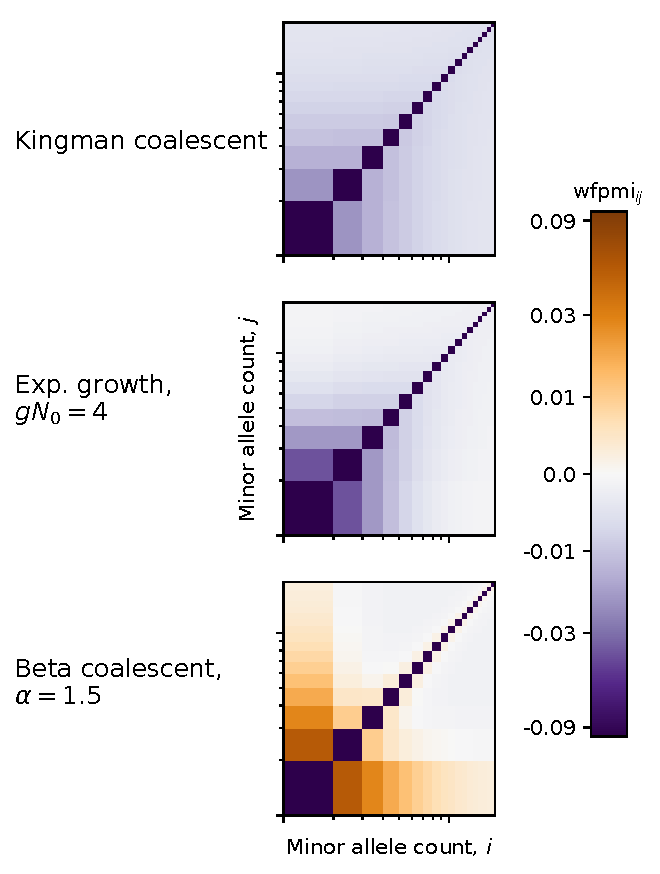
\includegraphics[width=0.5\textwidth]{figures/wfpmi_growth_beta.pdf}
\caption{Weighted frequency pointwise mutual information for three coalescent models: the time-homogeneous Kingman coalescent, the Kingman coalescent with exponential growth ($g=4$), and the beta coalescent ($\alpha=1.45$). For all models $n=39$. Growth and $\alpha$ parameters were chosen to generate average SFS with similar Tajima's D. The diagonal $i=j$ is masked. \label{fig:nonrecombining_pmi}}
\end{figure}

\Fig{fig:nonrecombining_pmi} shows the $\wfpmi$ for constant-$N$ Kingman coalescent; the Kingman coalescent with exponential growth, $N(t)=N_0 \exp(-g \frac{t}{N_0})$; and a beta coalescent intermediate between the Kingman and Bolthausen-Sznitman coalescents.
We find that while exponential growth with $g=4$ has a substantial effect on the SFS ($D = -0.39$), it does not qualitatively change the $\fpmi$.
In particular, $\fpmi_{i,j} < 0$ for all $i \neq j$, just as in the constant-$N$ Kingman coalescent.

On the other hand, a beta coalescent that generates similar distortions in the SFS ($\alpha=1.45$, $D = -0.42$) also generates positive $\fpmi$.
The effect of multiple mergers is strongest on $\fpmi$ between high and low minor allele counts.
This justifies coarse-graining the SFS and 2-SFS into high-- and low--minor allele count bins as defined above.

Accordingly, we computed the coarse-grained $\hilopmi$ between singletons and non-singletons ($i_c = 1$) for a range of $g$ and $\alpha$.
\Fig{fig:fpmi_vs_tajimasd} shows that as the population growth rate increases, distorting the SFS, $\hilopmi$ increases relative to the constant-$N$ Kingman, but plateaus at a negative value.
On the other hand, beta coalescents that generate similar distortions in the SFS, generate larger changes in $\hilopmi$, including positive values.
Thus, the 2-SFS in general, and $\hilopmi$ in particular, are capable of capturing the effects of multiple mergers beyond the distortions in branch lengths.

\begin{figure}
\centering
\includegraphics[width=0.8\textwidth]{figures/figure2.pdf}
\caption{Pointwise mutual information between singletons and non-singletons for Kingman coalescents with exponential growth and beta coalescents. The exponential growth rate, $g$, ranges from 0.25 to 8.0 in coalescent time units. The beta coalescent parameter, $\alpha$, ranges from 1.75 (nearly Kingman) to 1.25 (nearly Bolthausen-Sznitman). \label{fig:fpmi_vs_tajimasd}}
\end{figure}

\subsection*{Pointwise mutual information between recombining sites}

The previous sections have shown that $\fpmi$ between pairs of non-recombining sites can discriminate between the Kingman coalescent with population growth and the beta coalescent.
However, most demographic inference is performed on regions of the genome with non-zero recombination rates.
In fact, for large non-recombining loci, it is sometimes possible to reconstruct the gene genealogy exactly and calculate tree imbalance statistics directly (see e.g., \cite{Seger2010}).
The advantage of the $\fpmi$ approach is that it can be computed on a genomic scale, as with the SFS.
Therefore, it is important to assess the robustness of our approach to recombination between sites.

To measure the relationship between $\fpmi$ and recombination, we ran coalescent simulations using a version of the program \texttt{msprime} \cite{KehellerEtAl201?} modified to allow for multiple mergers (See Methods).
In particular, we simulated a model where the sizes of coalescent events are drawn from the distribution specified by the beta coalescent, as in our numerical calculations above.
In this model, marginal genealogies will follow the beta coalescent distribution, and the average SFS will be given by the formula in \cite{BirknerEtAl2013}.
We also simulated data from two models of population growth: exponential growth and a two-epoch piecewise-constant model.

\begin{figure}
\centering
\includegraphics[width=0.8\textwidth]{figures/figure4.pdf}
\caption{Weighted frequency pointwise information for three recombination rates with sample size $n=100$. As in \Fig{fig:nonrecombining_pmi}, the diagonal elements are masked, and the growth and multiple-merger parameters were chosen to generate average SFS with similar Tajima's D. \label{fig:wpmi_recombination}}
\end{figure}

\Fig{fig:wpmi_recombination} shows the weighted $\fpmi$ for three genetic distances in a constant-$N$ Kingman coalescent, a Kingman coalescent with exponential growth, and a beta coalescent.
As in the non-recombining case, the constant-$N$ and exponential-growth Kingman models have similar $\fpmi$.
In both models, $\fpmi > 0$ for $i\approx j$ for $r\E{T_2} \sim 1$.
This is presumably because trees at nearby sites contain clades with similar numbers of leaves.
These positive correlations, however, do not extend to $i \gg j$, which is the signal of multiple mergers in our coarse-grained $\hilopmi$.
On the other hand, the positive $\fpmi$ in the beta coalescent persists for $r\E{T_2} > 1$.

\begin{figure}
\centering
\includegraphics[width=0.8\textwidth]{figures/figure5.pdf}
\caption{Pointwise mutual information between high-- and low--minor allele count mutations ($\hilopmi$) versus genetic distance. The first three rows show coalescent simulations in \texttt{msprime}. Exponential growth rate $g$ ranges from 0.01 to 8.0 in coalescent time units. Piecewise constant change-points, range from 0.01 to 1 in coalescent time units, and the ratio of ancestral to modern population size ranges from 0.01 to 0.2. The fourth row shows forward-time \texttt{SLiM} simulations with selective sweeps at linked sites (beneficial mutation fraction $f_{\text{sel}} \in \{10^{-6}, 10^{-5}, 10^{-4}, 10^{-3}\}$, see Methods). Lines are colored by the distortion in the SFS, as measured by Tajima's D. [TODO: SPLIT SWEEPS PANELS OFF INTO THEIR OWN FIGURE.]\label{fig:hilo_vs_d}}
\end{figure}

\Fig{fig:hilo_vs_d} shows $\hilopmi(d,i_c)$ in both models of growth and the beta coalescent, for a range of $d=r\E{T_2}$ and three different choices of $i_c$.
Each curve represents a particular parameter combination and coalescent model and is colored by the distortion in the average SFS, which is independent of the recombination rate.
At low recombination rates, $\hilopmi$ may be greater in growing populations than in constant-$N$ populations (dotted lines), but is always less than zero, consistent with the results for non-recombining sites.
When $r\E{T_2}\geq 1$, $\hilopmi$ may be slightly positive for large $i_c$, but is smaller in growing populations than in the constant-$N$ Kingman model.
In all Kingman models, $\hilopmi$ decays to zero for $r\E{T_2}\gg 1$.

In contrast, the beta coalescent generates $\hilopmi$ that is consistently greater than the constant-$N$ Kingman.
As with non-recombining sites, the $\hilopmi$ is also greater in the beta coalescent model then in models of population growth than generate similar distortions in the SFS.
[IDEA: A plot of $\hilopmi$ at a fixed r vs Tajima's D for all the models together. Could make several plots, varying $r$ and $i_c$. This might be more convincing than the current figure.]
This is true across recombination rates and high/low cutoff minor allele counts.
These results demonstrate that $\hilopmi$ is capable of discriminating between coalescent models even when there is recombination between sites.

There is one other salient feature of \fig{fig:hilo_vs_d}: $\hilopmi$ does not decay to zero at long distances in the beta coalescent.
This is related to the results of \cite{EldonWakeley20??}, who showed that a model with ``jackpot'' reproductive events can generate infinite-range linkage disequilibrium.
They showed that different scalings of rates of mutation, pairwise coalescence, multiple merger coalescence, and recombination lead to different behaviors of diversity and linkage disequilibrium.
Our implementation of the beta coalescent model with recombination corresponds to a particular scaling limit where recombination does not have time to decorrelate trees during multiple mergers events, even at infinite genetic distances.
We do not expect this behavior to be universal to multiple mergers coalescents with recombination.

\subsection*{Linked selective sweeps}

Various authors have shown that natural selection can generate multiple merger coalescents at linked neutral sites (e.g., \cite{DurrettSchweinsberg2005, CoopRalph, NeherHallatscheck2013, DesaiEtAl, Seger}).
However, our simulations of the beta coalescent with recombination are of an explicitly neutral model.
Thus, they are at best an approximation to the selective models cited above.
It is therefore important to verify that selection at linked sites can, in fact, generate the sorts of signals in $\fpmi$ that we have detected in the beta coalescent.

To test this proposition, we performed forward-time simulations of recurring selective sweeps using the software \texttt{SLiM} \autocite{MesserEtAl201?}.
In these simulations, we simulated individual chromosomes with homogenous recombination and two types of mutations: neutral and beneficial with fixed selection coefficient $s$.
Both types of mutations occurred at random, uniformly distributed across the length of the chromosome.
By varying the recombination rate, mutation rates, population size, and selection coefficient, we were able to vary the rate of selective sweeps linked to neutral sites.
After the populations reached steady-state, we sampled individuals and calculated $\{\eta_i\}$ and $\{\eta_{ij}(d)\}$ for the neutral mutations.
(See Methods for details.)

The bottom row of \fig{fig:hilo_vs_d} shows the results of these simulations.
For intermediate genetic distances, $d r \E{T_2} \sim 1$, the effects of linked sweeps are qualitatively similar to the effects of the beta coalescent.
That is, when sweeps are sufficiently frequent to distort the SFS, as measured by Tajima's D, they also increase $\hilopmi$.
The primary difference between the forward-time sweeps and beta coalescent simulations, is that the distortions caused by sweeps decay to zero for $d r \E{T_2} \gg 1$.
This is reasonable because the effect of a particular sweep on genealogies should be localized around the beneficial mutation.

\subsection*{Coalescent model checking: application to \textit{Drosophila melanogaster}}

Our results above show that $\fpmi$ and its coarse-grained analog, $\hilopmi$ are useful for distinguishing population growth from the effects of multiple mergers.
This is true even when the population growth generates similar distortions in the SFS.
We therefore propose the following model-checking procedure for demographic inference methods
\begin{enumerate}[label=(\roman*), before=\unskip{: }]
    \item Fit a demographic model to data using any relevant method.
    \item Simulate genealogies under the fitted model (using \texttt{msprime} or other coalescent simulator). Calculate the $\fpmi(d)$ and $\hilopmi(d;i_c)$ predicted by the model.
    \item Calculate $\fpmi(d)$ and $\hilopmi(d;i_c)$ from the data.
    \item Compare true to predicted statistics. Evaluate model fit.
\end{enumerate}
This procedure checks whether the model is consistent with a dimension the data that was used in fitting the model.
Inconsistency suggests that the inferred $N(t)$ may be an artifact of natural selection, skewed offspring distributions, etc., rather than reflecting the true historical population size.

In this section, we illustrate the procedure just outlined by using genomic diversity data from the \textit{Drosophila melanogaster} DGPG3 panel \cite{LackEtAl2015}.
The DPGP3 data consists of haploid consensus sequences from $\sim 200$ wild-caught flies from a Zambian population known to be relatively free of cosmopolitan admixture.
Recently, several groups have used the DPGP3 data to estimate the population-size history of \textit{D. melanogaster} \autocite{TerhorstEtAl2017,RagsdaleGutenkunst2017}.
On the other hand, it is widely believed that the genetic diversity of \textit{Drosophila} is strongly shaped by natural selection (e.g., \cite{Elyashiv??201?, GarudPetrov2016, others?})
Thus, this data is a good candidate for demonstrating the utility of $\fpmi$ for assessing coalescent model fit.

After filtering for coverage, removing chromosome arms with known inversions, downsampling to $n=100$ samples per autosomal chromosome arm, and identifying 4-fold degenerate sites, we selected the central region of each chromosome that have consistent high diversity (Methods).
Because the average pairwise diversity varies between arms---possibly reflecting selection or different sets of segregating inversions---we performed all subsequent calculations on each arm independently.
We fit a demographic model to the site frequency spectra of these central regions using \texttt{fastNeutrino} \cite{BhaskarEtal2015}.
We fit a 3-epoch piecewise-constant model, with four free parameters: two changepoints and two population size ratios.
We report our fitted parameters in Table~\ref{tab:DPGP_params}.
We then simulated under our fitted model using \texttt{msprime} and computed the expected and observed SFS, $\fpmi$, and $\hilopmi$ (\fig{fig:dpgp3}, See methods for details.).

\begin{figure}
\centering
\includegraphics[width=0.8\textwidth]{figures/figure6.pdf}
\caption{DPGP3 data and coalescent model predictions. First row: observed (blue) and expected (orange) site frequency spectrum compared to constant-$N$ Kingman coalescent (dotted lines). Second row: Expected (upper triangle) and observed (lower triangle) weighted $\fpmi$ averaged over all pairs of sites less than $15 d_c$ apart. Third row: Observed (blue) and expected (orange) $\hilopmi$ versus genetic distance. Cutoff minor allele count, $i_c, = 5$. Solid blue curves show cubic spline fit. Dotted lines show the expectation under the constant-$N$ Kingman coalescent. [Middle row needs colorbar] \label{fig:dpgp3}}
\end{figure}

The first row of \fig{fig:dpgp3} shows that the expected SFS under the fit demographic models agree with the observed SFS, demonstrating that a time-varying $N(t)$ can explain this aspect of the data well.
In contrast, the second row shows the expected and observed weighted $\fpmi$ for averaged over distances less than $15 d_c$ apart, where $d_c = 2/ (\Pi \mu)$ is the distance scale corresponding to $r\E{T_2} = 1$.
Here, the data shows strong positive associations between nearby alleles at different frequencies, while the model of population growth predicts weak negative associations except just off of the diagonal.
This pattern extends across a range of genomic distances, $d/d_c \in (10^{-1}, 10^2)$ (\fig{fig:dpgp3}, third row).
As a result, we may conclude that the data is not well explained by the Kingman coalescent with population growth.

Note that the $\hilopmi$ decays toward zero at large distances.
This matches the expectation from simulations with selective sweeps rather than the beta coalescent.
However, we caution against concluding that sweeps are necessarily responsible for the deviations from the Kingman expectation.


\section*{Discussion}

\subsection*{Samples of four chromosomes}

\begin{figure}
\centering
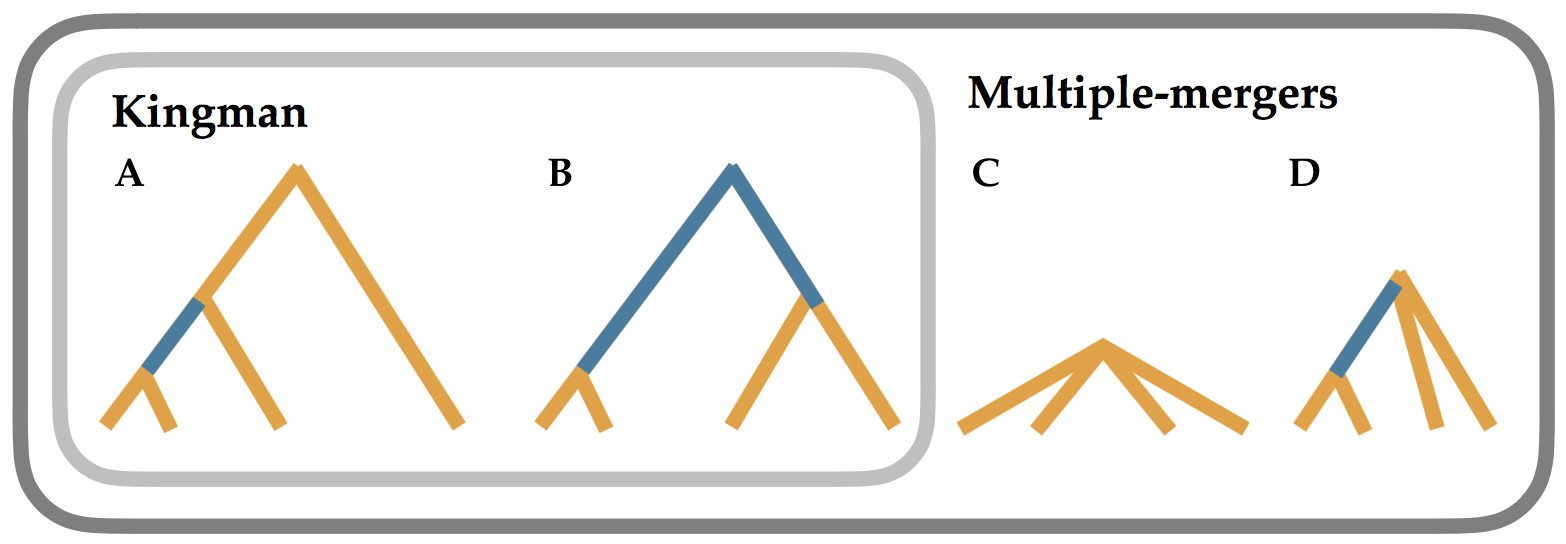
\includegraphics[width=0.8\textwidth]{figures/trees.png}
\caption{Genealogies with a sample size of $n=4$. Opportunities for singleton/tripleton mutations are in orange. Opportunities for doubletons are in blue. (Note: there is a third possible multiple-merger topology, not shown.) \label{fig:trees}}
\end{figure}

We can get an intuitive understanding for the result above by considering a sample four chromosomes.
In the Kingman coalescent, there are only two possible tree topologies (\Fig{fig:trees}).
Furthermore, the total branch length is independent of the topology \cite{Wakeley2009}.
As a result, there is a trade-off between the length of branches leading to singleton/tripleton mutations on one hand, and the branch length leading to doubletons on the other.
Genealogies with topology (A) will have more opportunities for the former and loci with topology (B) will have more opportunities for the latter.
Conditional on observing a doubleton at a site, it is thus more likely that the genealogy has topology (B) and so the expected number of singletons at sites with the same genealogy is lower than average.
In terms of the 2-SFS, we have $\E{\eta_{12}} < \E{\eta_{1}} \E{\eta_{2}}$.

On the other hand, multiple mergers induce correlations between the tree topology and the total branch length.
For example, topology (C) has less opportunity for singletons \emph{and} less opportunity for doubletons than (A) or (B), even though the expected proportion of singletons is higher.
Thus, observing \emph{any mutation at all} makes topology (C) less likely and the expected number of other mutations at all frequencies higher.
If multiple-mergers events are frequent enough, this effect may dominate the tradeoff between (A) and (B) so that $\E{\eta_{12}} > \E{\eta_{1}} \E{\eta_{2}}$.

\begin{figure}
\centering
\includegraphics[width=0.8\textwidth]{figures/figure3.pdf}
\caption{Distortions in $\fpmi$ vs. distortions in the SFS for $n=4$. Parameters for beta coalescents and exponential growth are as in \fig{fig:fpmi_vs_tajimasd}. For the piecewise-constant--$N$ model, the fold-change in $N$ varies from 2 to $2^4$ and the time of this change varies from $2^{-4}$ to 2 in coalescent time units. \label{fig:sdpmi_vs_sdratio}}
\end{figure}

As argued above, $\E{\eta_{12}}$ is also distorted by changes in the coalescent time distribution induced by population growth.
\Fig{fig:sdpmi_vs_sdratio} demonstrates that $\fpmi$ accounts for this fact by normalizing by the SFS.
\Fig{fig:sdpmi_vs_sdratio} plots $\fpmi_{12}$ against the ratio of singletons to doubletons $\eta_1 / \eta_2$ for the beta coalescent and two models of population growth: exponential growth and a piecewise-constant model with two epochs.
In the latter model, we vary both the fold-change in $N$ and the time of the change.
Like Tajima's D, the singleton/doubleton ratio measures distortion the SFS relative to the constant-$N$ Kingman coalescent.
(In fact, with $n=4$, this ratio captures \emph{all} of the distortion in the SFS.)
As with the larger sample size (\fig{fig:fpmi_vs_tajimasd}), mulitple mergers generate larger distortions in $\fpmi$ than population growth does, accounting for the distortions in the SFS.
Moreover, the two different models of growth collapse onto one another.
This suggests that for the Kingman coalescent with growth, $\fpmi_{12} \approx f(\eta_1/\eta_2)$ for some function $f$.

\begin{itemize}
    \item Review results.
    \item Availability of code: models for computing moments numerically, scripts for running simulations. Notebooks for data analysis.
    \item We focus here on coalescent-based methods, but also relevant for diffusion methods (because they imply a coalescent model)
    \item Mention methods to fit multiple mergers coalescent to data (computationally difficult). Not really what we're trying to do here. Our goal is that you can exploit this extra dimension of the data you already have to check your model and make sure you're not fitting a signal of selection, etc with a demographic model.
    \item Could also develop a formal hypothesis testing procedure, using the bootstrap, etc.
    \item Compare with: Single-locus tests that rely on building trees (Seger whale lice, Neher with viruses)
    \item Compare with: Multi-locus tests that compare a particular region to genomic background. (What if the background isn't neutral/Kingman?)
    \item But: we could extend our method to a local method that looks for variation in ``multiple-merger-ness''
    \item Multiple-mergers coalescent and recombination: open area of research
    \item $\fpmi(d)$ should be a standard posterior check for demographic models. Possibly incorporate into model fitting packages.
    \item Interesting to compare across species.
\end{itemize}

\printbibliography

\section*{Supplementary Methods}
[IF NECESSARY]

\clearpage

\section*{Supplementary Figures and Tables}

\begin{figure}[h!]
\centering
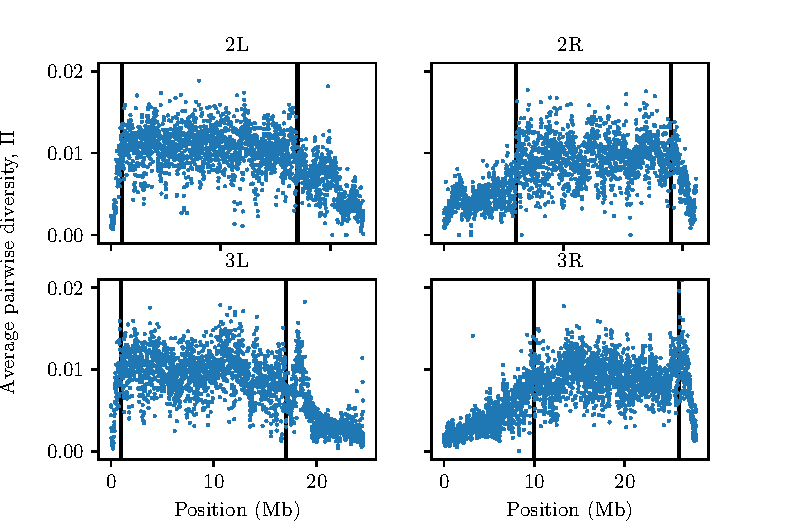
\includegraphics[width=0.8\textwidth]{figures/pi_vs_position.pdf}
\caption{Average pairwise diversity, $\Pi$, of 100 haploid samples from DPGP3 panel. Each point represents the average over a 10~KB window. Vertical lines show the boundaries of the central regions defined in Table~\ref{tab:central_regions}.
\label{fig:dpgp_pi}}
\end{figure}

\begin{table}[h!]
  \begin{center}
    \caption{Boundaries of the homogeneous central regions of chromosomes (shown in \ref{fig:dpgp_pi}).}
    \label{tab:central_regions}
    \begin{tabular}{l|r|r} % <-- Alignments: 1st column left, 2nd middle and 3rd right, with vertical lines in between
      \textbf{Chr.} & \textbf{Start position (MB)} & \textbf{End position (MB)}\\
      \hline
      2L & 1 & 17\\
      2R & 6 & 19\\
      3L & 1 & 17\\
      3R & 10 & 26
    \end{tabular}
  \end{center}
\end{table}

\begin{table}[h!]
  \begin{center}
    \caption{Fraction of sites with at least 90 genotyped samples}
    \label{tab:called_sites}
    \begin{tabular}{l|r|r} % <-- Alignments: 1st column left, 2nd middle and 3rd right, with vertical lines in between
      \textbf{Chr.} & \textbf{All sites} & \textbf{Polymorphic sites}\\
      \hline
      2L & 0.913 & 0.924 \\
      2R & 0.922 & 0.925 \\
      3L & 0.919 & 0.920 \\
      3R & 0.933 & 0.936
    \end{tabular}
  \end{center}
\end{table}

\begin{table}[h!]
  \begin{center}
    \caption{Piecewise-constant model parameters fit to the SFS of each chromosome arm (see \eq{eq:piecewise}, $N_{\text{anc}}=3 \times 10^5$).}
    \label{tab:DPGP_params}
    \begin{tabular}{l|r|r|r|r} % <-- Alignments: 1st column left, 2nd middle and 3rd right, with vertical lines in between
        \textbf{Chr.} & \textbf{$N_1 (\times 10^5)$} & \textbf{$N_2 (\times 10^5)$} & \textbf{$t_1 (\times 10^4)$} & \textbf{$t_2 (\times 10^4)$}\\
        \hline
        2L & 10.7 & 4.6 & 2.8 & 39.9 \\
        2R &  9.1 & 3.9 & 1.6 &  8.8 \\
        3L &  7.3 & 3.8 & 1.3 &  6.4 \\
        3R &  9.7 & 5.1 & 2.2 &  8.6
    \end{tabular}
  \end{center}
\end{table}

\end{document}

TODO:
- Abstract
- Discussion
- Edit figures
- Consistency of nomenclature, labeling, etc.
- Check drosophila numbers. Get citations or remake figure.
- Check references to Methods. (Should all be there and all have corresponding methods section.)
- Get rest of citations
- Code:
    - organize
    - clean
    - comment
    - post on Github

Things that were done but not included in this ms:
- Background selection (didn't run the right parameters to see the effect. Might be computationally challenging.)
- 2-Deme model with migration. (Could include in SI.)
- 1-D stepping-stone.

OLD TEXT:
% Tests of the standard Kingman coalescent based on the SFS originated with \cite{Tajima1989}, \cite{FuLi1993}, and \cite{SimonsenEtAl1995} (see \cite{Achaz2009} for a unifying framework).

% There are two limitations of these existing results.
% First, they only apply to time-homogeneous coalescent processes and thus do not distinguish between multiple-mergers coalescents and Kingman models with time-varying population size.
% Second, they assume a non-recombining locus and may break down for sites separated by a finite genetic distance.

% With modern population genomics data sets, full-data likelihood models are impractical, so population-size inference is typically done on informative summary statistics.
% One widely used statistic is the site frequency spectrum (SFS): the number of mutations observed as a function of their allele frequency in the sample.
% The expected number of mutations at a given frequency depends on the branch lengths, and hence, on the coalescent rate.
% Thus, one can infer the coalescent rate by integrating over tree topologies, weighted by their probabilities under the Kingman coalescent.
% Some methods perform this integration by Monte Carlo simulation (e.g., \cite{CoventryEtAl2010, ExcoffierEtAl2013}).
% Others (e.g., \cite{Nielsen2000}, \cite{BhaskarEtAl2015}), compute the expected site frequency spectrum directly for simple demographic models using the results of \cite{GriffithsTavare1998} or \cite{PolanskiKimmel2003}.
% (Another class of SFS-based methods are based on corresponding forward-time models rather than the coalescent \autocite{GutenkunstEtAl2009, LukicEtAl2011, RagsdaleGutenkunst2017, JouganousEtAl2017}.)
